% !TEX program = pdflatex
\documentclass[11pt,a4paper]{amsart}

% --- ENCODING & FONTS ------------------------------------------------------
\usepackage[utf8]{inputenc}
\usepackage[T1]{fontenc}

% --- MATH PACKAGES ---------------------------------------------------------
\usepackage{amsmath,amssymb,amsthm,mathtools}
\usepackage{graphicx}

% --- PAGE LAYOUT -----------------------------------------------------------
\usepackage{geometry}
\geometry{a4paper,left=25mm,right=25mm,top=25mm,bottom=30mm}
\usepackage{lastpage}
\usepackage{refcount}

% --- HYPERLINKS ------------------------------------------------------------
\usepackage[hyphens]{url}
\usepackage[colorlinks=true, urlcolor=blue, linkcolor=blue]{hyperref}
\usepackage{orcidlink}
\usepackage{eso-pic}
\usepackage{doi}

\hypersetup{
    pdftitle={From Trial Division to Smooth Prime Indicators: A Framework Based on Fourier Series},
    pdfauthor={Sebastian Fuchs (ORCID: 0009-0009-1237-4804)},
    pdfkeywords={Prime numbers, analytic prime indicator, analytic number theory, divisor function, sum-of-divisors function, tau function, sigma function, trigonometric series, Fejér kernel},
    pdfsubject={Primary 11A41;
Secondary 11L03, 42A10}
}

% --- MACROS & THEOREMS -----------------------------------------------------
\newcommand{\Px}{\mathcal{P}}
\newcommand{\R}{\mathbb{R}}

% --- THEOREM STYLES --------------------------------------------------------
\theoremstyle{plain}
\newtheorem{theorem}{Theorem}[section]
\newtheorem{conjecture}[theorem]{Conjecture}
\newtheorem{lemma}[theorem]{Lemma}
\newtheorem{property}[theorem]{Property}
\theoremstyle{definition}
\newtheorem{definition}[theorem]{Definition}


% --- METADATA --------------------------------------------------------------
\title[From Trial Division to Smooth Prime Indicators]{From Trial Division to Smooth Prime Indicators: A Framework Based on Fourier Series}
\author{Sebastian Fuchs \orcidlink{0009-0009-1237-4804}}
\address{Institut für Informatik, Humboldt-Universität zu Berlin, 10099 Berlin, Germany}
\email{\href{mailto:sebastian.fuchs@hu-berlin.de}{sebastian.fuchs@hu-berlin.de}}
\date{June 26, 2025}
\subjclass[2020]{Primary 11A41;
Secondary 11L03, 42A10}
\keywords{Prime numbers, analytic prime indicator, analytic number theory, divisor function, sum-of-divisors function, tau function, sigma function, trigonometric series, Fejér kernel}

% ---------------------------------------------------------------------------
\begin{document}

\begin{abstract}
This work introduces a flexible framework for constructing smooth ($C^\infty$) analogues of classical arithmetic functions, based on the smoothing of a trigonometric representation of trial division.
A foundational function $\Px\colon\R\to\R$ of class $C^1$ is first presented, whose zeros for $x>2$ correspond precisely to the odd primes.
The fact that this function is of class $C^1$ but not smoother motivates its generalization into a versatile framework for constructing fully smooth ($C^\infty$) analogues.
This framework is then applied to construct two novel functions: a smooth analogue of the divisor-counting function, $\Px_{\tau}$, and a smooth analogue of the sum-of-divisors function, $\Px_{\sigma}$.
Both functions are proven to be of class $C^\infty$. It is shown that these new constructions possess a complete prime-zero property for all integers $x \ge 2$.
The robustness of this property for real numbers is analyzed for each function.
It is demonstrated that $\Px_{\tau}$ provides a robust prime indicator for all real numbers, while the properties of $\Px_{\sigma}$ in this regard lead to an open question concerning the existence of non-integer zeros.
The construction methodology, properties, and potential of these functions are discussed in detail.
\end{abstract}

\maketitle

% ---------------------------------------------------------------------------
\section{Introduction}
Prime numbers occupy a central position in number theory, and explicit functions that identify primes have long been a subject of mathematical inquiry~\cite{hardy2008}.
Seminal early results include the non-constructive formula of Mills, which relies on the existence of a special constant~\cite{mills1947}, and the explicit but computationally infeasible formula of Willans, which is based on Wilson's theorem~\cite{willans1964}.
The construction of such functions continues to be an active area of research.
Modern approaches are diverse, ranging from purely arithmetic constructions~\cite{mazzanti2024} to various forms of analytic indicators~\cite{helfgott2023, hiary2018, seriprim2022}.
A recent focus has been the development of smooth, differentiable functions that approximate the characteristic function of the primes, for instance through integral kernel methods~\cite{semenov2025}.
This note contributes to this line of inquiry by introducing a new type of analytic prime indicator derived from first principles of Fourier analysis.
The approach presented here is distinct from several other modern methods.
Unlike indicators based on integral kernel methods~\cite{semenov2025} or purely arithmetic constructions~\cite{mazzanti2024}, the present work uses the Fejér kernel—a classical tool for ensuring the convergence of trigonometric series~\cite{zygmund2002}—to regularise a trigonometric representation of trial division.
This approach offers a direct and constructive path to an initial $C^1$ function whose analytical properties can be precisely controlled.
The main contribution of this paper is to show that this initial idea can be extended into a general framework capable of generating smooth ($C^\infty$) analogues of various classical arithmetic functions that possess a complete prime-indicating property for all integers $x \ge 2$.
This paper is organized as follows. Section~2 introduces the foundational function $\Px(x)$ and its construction.
Sections~3, 4, and 5 detail its analytic properties, its prime-zero property for odd primes, and its quantitative behavior, respectively.
These sections establish the groundwork and motivation for generalization. Section~6 introduces the general framework, including a highly refined smooth cutoff function.
Sections~7 and 8 apply this framework to construct a smooth divisor-counting function ($\Px_{\tau}$) and a smooth sum-of-divisors function ($\Px_{\sigma}$), analyzing their properties and their complete prime-zero property in detail.
Section~9 discusses an application of the foundational function to the prime-counting function $\pi(x)$, and Section~10 provides concluding remarks and discusses future research directions.
Throughout, $\lceil t \rceil$ denotes the ceiling of a real number~$t$.
Numerical verifications of the key properties and the plots presented in this paper is maintained in a public repository.\footnote{The repository is available at: \url{https://github.com/SebastianFoxxx/analytic-prime-indicator}}
% ---------------------------------------------------------------------------
\section{Analytic construction of $\Px$}

\subsection{Motivation}\label{subsec:motivation}
Trial division classifies an integer $x$ as composite once a divisor $i\le\sqrt{x}$ is found.
This principle can be translated into an analytical form by constructing a quotient $Q(x,i)$ that probes the divisibility of $x$ by $i$.
The numerator, $\sin^2(\pi x)$, serves as a detector for integers, as it vanishes precisely for $x \in \mathbb{Z}$.
The denominator, $\sin^2(\pi x/i)$, can be interpreted as a measure of a "relative divisibility remainder": it approaches zero when $x/i$ is near an integer (i.e., when $i$ is "almost" a divisor of $x$) and is large otherwise.
The resulting quotient,
\[
Q(x,i)=\frac{\sin^{2}(\pi x)}{\sin^{2}(\pi x/i)},
\]
thus relates the integer nature of $x$ to its divisibility by $i$.
For an integer $x$, this expression conveniently vanishes if $i$ is not a divisor.
However, this form becomes indeterminate ($0/0$) at the most crucial points: where $i$ is a true divisor of $x$.
The goal is therefore to regularise this expression to resolve the indeterminacy while preserving its underlying prime-indicating property.
The Fejér identity, a classical tool for ensuring the convergence of Fourier series, provides a direct way to resolve such trigonometric indeterminacies.
\subsection{Regularisation}
Invoking the Fejér identity
\[
\frac{\sin^{2}(ny)}{\sin^{2}y}=n+2\sum_{k=1}^{n-1}(n-k)\cos(2ky)
\]
with $n=i$ and $y=\pi x/i$ removes the indeterminacy and yields a finite cosine sum that extends $Q$ to real~$x$.
\subsection{Definition}
The regularised function is constructed by summing the Fejér-kernel-based terms over all potential divisors up to $\sqrt{x}$.
For clarity, let $F(x,i)$ denote the Fejér kernel term:
\begin{equation}\label{eq:Fxi}
F(x,i) = i+2\sum_{k=1}^{i-1}(i-k)\cos\left(\frac{2\pi k x}{i}\right).
\end{equation}
\begin{definition}\label{def:Px}
For $x>1$ the function $\Px(x)$ is defined as
\begin{equation}\label{eq:Px}
\Px(x)=\frac{1}{x}\sum_{i=2}^{\lceil\sqrt{x}\rceil} F(x,i),
\end{equation}
and $\Px(x)=0$ is set for $x\le1$.
\end{definition}
For brevity, let $N(x) = \lceil\sqrt{x}\rceil$ denote the upper summation limit.
% ---------------------------------------------------------------------------
\section{Smoothness properties of $\Px$}

\subsection{Global $C^{1}$-smoothness}
\begin{property}\label{prop:C1}
The function $\Px$ is continuous on $\R$ and of class $C^1$ for $x>0$.
\end{property}
\begin{proof}
On any open interval $((m-1)^2, m^2)$ for $m\ge 2$, the summation limit $\lceil\sqrt{x}\rceil$ is fixed at $m$, making $\Px$ a finite sum of $C^\infty$ functions and thus $C^\infty$ on these intervals.
The critical points are the integer squares $x=m^2$, where the limit jumps from $m$ to $m+1$.
First, continuity at $x=m^2$ is established. As $x \to (m^2)^-$, the function is $\Px(x) = \frac{1}{x}\sum_{i=2}^{m} F(x,i)$.
As $x \to (m^2)^+$, an additional term $\frac{1}{x}F(x,m+1)$ appears. Continuity requires this new term to be zero at the transition point.
At $x=m^2$, the argument of the cosine in $F(m^2, m+1)$ becomes $\frac{2\pi k m^2}{m+1} = 2\pi k(m-1) + \frac{2\pi k}{m+1}$.
Thus,
\[ F(m^2, m+1) = (m+1) + 2\sum_{k=1}^{m}(m+1-k)\cos\left(\frac{2\pi k}{m+1}\right). \]
This is the Fejér kernel $K_m(t)$ evaluated at $t=2\pi/(m+1)$, which equals $\frac{\sin^2((m+1)t/2)}{\sin^2(t/2)} = \frac{\sin^2(\pi)}{\sin^2(\pi/(m+1))} = 0$ for $m \ge 1$.
The added term $\frac{1}{m^2}F(m^2, m+1)$ is zero, proving continuity.

Next, $C^1$-smoothness is established.
The derivative $\Px'(x)$ exists on the open intervals. For $\Px$ to be of class $C^1$ at $x=m^2$, equality of the left-sided and right-sided limits of $\Px'(x)$ is required.
This is equivalent to showing that the derivative of the newly added term, $\frac{d}{dx}\left[\frac{1}{x}F(x, m+1)\right]$, vanishes at $x=m^2$.
By the quotient rule, this derivative is $\frac{x F'(x, m+1) - F(x, m+1)}{x^2}$.
Since $F(m^2, m+1)=0$, it is only necessary to show that $F'(m^2, m+1)=0$, where the derivative is with respect to $x$.
The derivative with respect to $x$ is:
\[ F'(x, i) = \frac{\partial}{\partial x}\left[i+2\sum_{k=1}^{i-1}(i-k)\cos\left(\frac{2\pi k x}{i}\right)\right] = -\frac{4\pi}{i}\sum_{k=1}^{i-1}k(i-k)\sin\left(\frac{2\pi k x}{i}\right).
\]
Evaluating at $x=m^2$ and $i=m+1$:
\[ F'(m^2, m+1) = -\frac{4\pi}{m+1}\sum_{k=1}^{m}k(m+1-k)\sin\left(\frac{2\pi k m^2}{m+1}\right).
\]
Using $\frac{m^2}{m+1} = m-1 + \frac{1}{m+1}$, the sine term becomes $\sin\left(2\pi k(m-1) + \frac{2\pi k}{m+1}\right) = \sin\left(\frac{2\pi k}{m+1}\right)$.
The sum is $S = \sum_{k=1}^{m}k(m+1-k)\sin\left(\frac{2\pi k}{m+1}\right)$. Let $a_k = k(m+1-k)\sin\left(\frac{2\pi k}{m+1}\right)$.
For $1 \le k \le m$, let its partner term be indexed by $j = m+1-k$.
Note that $1 \le j \le m$ as well. The $j$-th term is:
\begin{align*} a_{m+1-k} &= (m+1-k)(m+1-(m+1-k))\sin\left(\frac{2\pi (m+1-k)}{m+1}\right) \\ &= (m+1-k)k\sin\left(2\pi - \frac{2\pi k}{m+1}\right) \\ &= -k(m+1-k)\sin\left(\frac{2\pi k}{m+1}\right) = -a_k.
\end{align*}
Therefore, $a_k + a_{m+1-k} = 0$. The summation range is now considered.
If $m+1$ is odd, $k$ can never equal $m+1-k$, so all $m$ terms can be perfectly paired into $m/2$ pairs that sum to zero.
If $m+1$ is even, say $m+1=2N$, there is a middle term where $k=m+1-k$, which occurs at $k=N$.
For this term, the sine part is $\sin(2\pi N / (2N)) = \sin(\pi) = 0$, so $a_N=0$.
All other terms pair up and sum to zero. In all cases, the total sum $S$ is zero.
Thus, $F'(m^2, m+1) = 0$, which ensures the derivative is continuous across the integer squares.
\end{proof}

\subsection{Second-derivative jumps}
\begin{property}\label{prop:second}
$\Px''$ has jump discontinuities at each integer square $x=m^2$, for $m\ge2$.
\end{property}
\begin{proof}
The jump is caused by the second derivative of the term $\frac{1}{x}F(x, m+1)$, which is added to the definition of $\Px(x)$ as $x$ crosses $m^2$.
Since the term itself and its first derivative are zero at $x=m^2$, the magnitude of the jump in $\Px''(x)$ is precisely the value of this term's second derivative at that point.
A calculation shows that $\frac{d^2}{dx^2}\left[\frac{F(x,m+1)}{x}\right]_{x=m^2} = \frac{F''(m^2, m+1)}{m^2}$. The second derivative of the Fejér term is $F''(x, i) = -\frac{8\pi^2}{i^2}\sum_{k=1}^{i-1}k^2(i-k)\cos\left(\frac{2\pi k x}{i}\right)$.
At $x=m^2$ and $i=m+1$, this becomes $F''(m^2, m+1) = -\frac{8\pi^2}{(m+1)^2}\sum_{k=1}^{m}k^2(m+1-k)\cos\left(\frac{2\pi k}{m+1}\right)$, which is in general non-zero.
For instance, for $m=2$ (the jump at $x=4$), a direct calculation yields $F''(4, 3) = -\frac{8\pi^2}{9} \sum_{k=1}^{2}k^2(3-k)\cos\left(\frac{2\pi k}{3}\right) = -\frac{8\pi^2}{9}(1^2\cdot 2 \cdot (-\frac{1}{2}) + 2^2\cdot 1 \cdot (-\frac{1}{2})) = \frac{8\pi^2}{3} \neq 0$.
This non-vanishing contribution causes the jump discontinuity, which is a direct consequence of the sharp cutoff in the summation at $i = \lceil\sqrt{x}\rceil$.
\end{proof}

% ---------------------------------------------------------------------------
\section{The Prime-Zero Property of the Foundational Function $\Px(x)$}

The main result for the foundational function $\Px(x)$ establishes that it acts as an indicator for odd prime numbers.
This property is formalized in the following theorem.

\begin{theorem}[Odd Prime-Zero Property of $\Px(x)$]\label{thm:primezero}
For all real $x>2$, the function $\Px(x)$ has the property
\[
\Px(x)=0 \quad\Longleftrightarrow\quad x \text{ is an odd prime}.
\]
Furthermore, for all non-prime $x>2$, $\Px(x) > 0$.
\end{theorem}

\begin{proof}
The property is proven by considering three exhaustive cases for $x > 2$.
\begin{enumerate}
  \item \textbf{Case 1: Let $x = p$, where $p$ is an odd prime.}
  The sum for $\Px(p)$ runs from $i=2$ to $\lceil\sqrt{p}\rceil$.
  For any integer $i$ in this range, by the definition of a prime number, $i$ is not a divisor of $p$.
  The term $F(p, i)$ is thus given by the non-singular form of the Fejér kernel, $F(p, i) = \frac{\sin^2(\pi p)}{\sin^2(\pi p/i)}$.
  Since $p$ is an integer, the numerator $\sin^2(\pi p) = 0$.
  Since $i$ is not a divisor of $p$, the denominator $\sin^2(\pi p/i) \neq 0$.
  Thus, $F(p, i) = 0$ for all $i$ in the sum. Consequently, $\Px(p) = \frac{1}{p}\sum 0 = 0$.
  \item \textbf{Case 2: Let $x = n$, where $n$ is a composite integer.}
  Since $n$ is composite, there exists at least one integer divisor $d$ with $2 \le d \le \sqrt{n}$.
  The sum for $\Px(n)$ includes the term $F(n, d)$. For this term, the cosine sum definition must be used as the equivalent quotient form is indeterminate.
  The argument of the cosine is $\frac{2\pi k n}{d}$, which is an integer multiple of $2\pi$ because $d$ divides $n$.
  Thus, $\cos(\frac{2\pi k n}{d}) = 1$ for all $k$. The term becomes
  \[ F(n, d) = d + 2\sum_{k=1}^{d-1}(d-k) = d + 2\left(\frac{(d-1)d}{2}\right) = d^2.
  \]
  All other terms $F(n, i)$ for which $i$ is not a divisor of $n$ are zero, as shown in Case 1. The total sum $\sum_{i=2}^{\lceil\sqrt{n}\rceil} F(n, i)$ is therefore a sum of zeros and at least one positive term $d^2$.
  The sum is strictly positive, and thus $\Px(n) = \frac{1}{n} \sum F(n, i) > 0$.
  \item \textbf{Case 3: Let $x \in \mathbb{R} \setminus \mathbb{Z}$ (x is a non-integer).}
  For a non-integer $x$, $\sin^2(\pi x) > 0$.
  Furthermore, for any integer $i \ge 2$, the fraction $x/i$ is not an integer, so $\sin^2(\pi x/i) \neq 0$.
  The function $\Px(x)$ can thus be written using the quotient form for every term:
  \[ \Px(x) = \frac{1}{x} \sum_{i=2}^{\lceil\sqrt{x}\rceil} \frac{\sin^2(\pi x)}{\sin^2(\pi x/i)} = \frac{\sin^2(\pi x)}{x} \left( \sum_{i=2}^{\lceil\sqrt{x}\rceil} \frac{1}{\sin^2(\pi x/i)} \right).
  \]
  For $x>2$, all three factors are positive: $\frac{1}{x} > 0$, $\sin^2(\pi x) > 0$, and the summation term is a sum of strictly positive numbers.
  Therefore, $\Px(x) > 0$.
\end{enumerate}
These three cases combined show that for all $x>2$, $\Px(x)=0$ if and only if $x$ is an odd prime, and is positive otherwise.
\end{proof}

% ---------------------------------------------------------------------------
\section{Quantitative Properties and Complexity of $\Px(x)$}

\subsection{Lower Bound for Composite Integers}
A crucial property for applications is a quantitative lower bound on $\Px(n)$ for composite integers $n$.
From the proof of Theorem~\ref{thm:primezero}, it is known that $\Px(n)>0$ for composite $n$.
More explicitly, the value is given by
\[ \Px(n) = \frac{1}{n} \sum_{\substack{d|n \\ 2 \le d \le \sqrt{n}}} d^2.
\]
Let $p_1$ be the smallest prime factor of $n$. Then $p_1 \le \sqrt{n}$, and the sum must contain at least the term $p_1^2$.
The smallest possible prime factor for any composite number is 2. Therefore, a universal lower bound is established by considering the worst-case scenario:
\[ \Px(n) \ge \frac{p_1^2}{n} \ge \frac{2^2}{n} = \frac{4}{n}.
\]
This lower bound is sharp and is attained for numbers of the form $n=2p$ where $p$ is a prime greater than 2. This inverse relationship with $n$ is a key feature of the indicator.
\subsection{Computational Complexity}
The evaluation of $\Px(x)$ for a given $x>1$ requires computing a double summation.
The outer sum runs up to $N(x) = \lceil\sqrt{x}\rceil$, and the inner sum for each $i$ runs up to $i-1$.
The total number of cosine evaluations is approximately
\[ \sum_{i=2}^{N(x)} (i-1) = \frac{(N(x)-1)N(x)}{2} \approx \frac{x}{2}.
\]
Therefore, the computational complexity of evaluating $\Px(x)$ is $O(x)$.

% ---------------------------------------------------------------------------
\section{A General Framework for Smooth Analogues of Arithmetic Functions}

\subsection{Motivation}
The function $\Px(x)$ achieves its prime-indicating property at the cost of limited smoothness.
The discontinuities in its second derivative are a direct result of the sharp cutoff in the summation limit $\lceil\sqrt{x}\rceil$.
To create globally smooth ($C^\infty$) functions, this sharp cutoff must be replaced with a smooth one, transforming the finite sum into a rapidly converging infinite series.
More importantly, the underlying structure of $\Px(x)$ can be generalized.
The value of $\Px(n)$ for a composite integer $n$ is $\frac{1}{n}\sum d^2$, which is not immediately intuitive.
This motivates a generalization to create smooth functions that correspond to more classical arithmetic functions, such as the divisor-counting function $\tau(n)$ (the number of positive divisors of $n$) or the sum-of-divisors function $\sigma(n)$ (the sum of positive divisors of $n$).
This section introduces a general framework to achieve this.

\subsection{The Framework Structure}
A generalized structure for a smooth function is proposed as:
\[ \Px_W(x; k) = \sum_{i=2}^{\infty} \phi_{\text{mod}}\left(\frac{i}{x+1}; k\right) \cdot W(i) \cdot F(x,i) \]
where $F(x,i)$ is the Fejér term from \eqref{eq:Fxi}, $W(i)$ is a **weighting function** that determines the arithmetic property of the resulting function, and $\phi_{\text{mod}}$ is an optimized smooth cutoff function.
\subsection{An Optimized Smooth Cutoff Function}
To achieve the desired properties, a cutoff function is needed that is essentially 1 for its argument $u \le 1$ and decays rapidly for $u > 1$.
This allows for the accurate inclusion of all relevant terms up to $i \approx x$ while ensuring convergence of the infinite sum.
A function based on the hyperbolic tangent provides these properties and is of class $C^\infty$.
\begin{definition}[Smooth Transition Cutoff Function]
Let $k>0$ be a steepness parameter. The modified cutoff function $\phi_{\text{mod}}\colon\R\to(0,1)$ is defined as
\begin{equation}\label{eq:phimod}
\phi_{\text{mod}}(u; k) = \frac{1 - \tanh\big(k \cdot (u - 1)\big)}{2}.
\end{equation}
\end{definition}
This function provides a smooth transition from 1 to 0 centered at $u=1$.
For a large $k$ (e.g., $k \ge 50$), it acts as a very close approximation to a step function, being nearly 1 for $u<1$ and nearly 0 for $u>1$, while remaining $C^\infty$.
The argument to this function is chosen as $i/(x+1)$ to ensure that for any integer $x=n$, all divisors $d \le n$ result in an argument $d/(n+1) < 1$, thereby receiving a weight of almost exactly 1.

% ---------------------------------------------------------------------------
\section{Application 1: A Smooth Divisor-Counting Function (\texorpdfstring{$\Px_{\tau}$}{P_tau})}

\subsection{Motivation and Construction}
The first goal is the construction of a smooth function that, for an integer $n$, counts its divisors.
From Theorem~\ref{thm:primezero}, it is known that for a divisor $d$ of an integer $n$, the Fejér term $F(n,d)$ evaluates to $d^2$.
To obtain a count of 1 for each divisor, this term is naturally normalized by $d^2$.
This motivates the choice of the weighting function $W(i) = 1/i^2$.
\begin{definition}[Smooth Divisor-Counting Function]
For $x>0$ and a steepness parameter $k>0$, the smooth divisor-counting analogue $\Px_{\tau}(x; k)$ is defined as
\begin{equation}\label{eq:Ptau}
\Px_{\tau}(x; k) = \left( \sum_{i=2}^{\infty} \phi_{\text{mod}}\left(\frac{i}{x+1}; k\right) \cdot \frac{F(x,i)}{i^2} \right) - 1,
\end{equation}
where $\phi_{\text{mod}}$ is given by \eqref{eq:phimod} and $F(x,i)$ by \eqref{eq:Fxi}.
\end{definition}
The final subtraction of 1 is included to establish a complete prime-zero property.
\subsection{Properties of $\Px_{\tau}$}

\begin{property}[Smoothness and Integer-Value Approximation]
The function $\Px_{\tau}(x;k)$ is of class $C^\infty$ for all $x>0$.
For any integer $n\ge2$, its value approximates the number of non-trivial divisors:
\[ \lim_{k\to\infty} \Px_{\tau}(n; k) = \tau(n)-2, \]
where $\tau(n)$ is the number of positive divisors of $n$.
\end{property}
\begin{proof}
The $C^\infty$-smoothness follows from standard arguments for series of smooth functions.
The function $\phi_{\text{mod}}$ is $C^\infty$, and its exponential decay for large arguments is sufficient to overcome the polynomial growth of the term $F(x,i)/i^2$, ensuring uniform convergence for all series of derivatives.
For an integer $n$, the term $F(n,i)/i^2$ is 1 if $i$ is a divisor of $n$ and 0 otherwise.
The sum becomes $\sum_{d|n, d\ge2} \phi_{\text{mod}}(d/(n+1);k)$. Since $d \le n$, the argument $d/(n+1) < 1$.
As $k\to\infty$, $\phi_{\text{mod}}(u;k) \to 1$ for all $u<1$. Thus, each divisor $d$ from 2 to $n$ contributes exactly 1 to the sum.
The total sum is therefore $\tau(n)-1$. After subtraction of 1, the result is $\tau(n)-2$.
\end{proof}

\begin{property}[Integer Prime-Zero Property of $\Px_{\tau}$]\label{prop:integerprimezero}
For any integer $n \ge 2$ and a sufficiently large steepness parameter $k$, the function $\Px_{\tau}(n; k)$ has the property
\[
\lim_{k\to\infty} \Px_{\tau}(n; k) = 0 \quad\Longleftrightarrow\quad n \text{ is a prime number}.
\]
For composite integers $n$, $\lim_{k\to\infty} \Px_{\tau}(n; k) > 0$.
\end{property}
\begin{proof}
Let $S_{\tau}(n;k)$ be the summation part of $\Px_{\tau}(n;k)$.
The analysis considers the limit $k\to\infty$.
\begin{enumerate}
    \item \textbf{Case 1: $n = p$ (a prime number, $p \ge 2$).}
    In the limit $k\to\infty$, the sum $\sum_{d|p, d\ge2} \phi_{\text{mod}}(d/(p+1);k)$ contains only one term for the divisor $d=p$.
    Since $p/(p+1) < 1$, the term $\phi_{\text{mod}}(p/(p+1);k)$ approaches 1. The Fejér term $F(p,p)/p^2$ is exactly 1. Thus, $\lim_{k\to\infty} S_{\tau}(p;k) = 1$, which results in $\lim_{k\to\infty} \Px_{\tau}(p;k) = 1-1 = 0$.
    This holds for $p=2$ as well.
    \item \textbf{Case 2: $n$ is a composite number, $n \ge 4$.}
    The sum becomes $\sum_{d|n, d\ge2} 1 = \tau(n)-1$.
    Since $n$ is composite, $\tau(n)\ge3$, so the sum is at least 2. Thus, $\lim_{k\to\infty} \Px_{\tau}(n;k) = (\tau(n)-1)-1 = \tau(n)-2 \ge 1 > 0$.
\end{enumerate}
This establishes the property for all integers $n \ge 2$.
\end{proof}

\begin{conjecture}[Robustness for Real Numbers]\label{conj:Ptau_real}
For a sufficiently large steepness parameter $k$, the function $\Px_{\tau}(x; k)$ is non-zero for all non-prime real numbers $x \ge 2$.
Specifically, it is conjectured that $\Px_{\tau}(x; k) > 0$ for non-integer $x > 3$.
\end{conjecture}

\subsubsection*{Heuristic Argument for Conjecture~\ref{conj:Ptau_real}}
The robustness of the non-zero property for non-integer $x$ is supported by analyzing the behavior of $\Px_{\tau}(x; k)$ at its likely local minima, which occur near integers.
Let $S_{\tau}(x;k)$ be the summation part of $\Px_{\tau}$.
For a non-integer $x > 3$, every term in the sum defining $S_{\tau}(x;k)$ is strictly positive.
A strong indication for $S_{\tau}(x;k) > 1$ (and thus $\Px_{\tau}(x;k) > 0$) comes from examining the neighborhoods of integers $n \ge 4$.
For an even integer $n$, as $x \to n$, the term $F(x,2)/4 \approx \cos^2(\pi x/2)$ approaches 1. Since all other terms are positive, $S_{\tau}(x;k)$ must exceed 1 in this neighborhood.
For an odd integer $n \ge 5$, as $x \to n$, the term $F(x,n)/n^2$ approaches 1 (via L'Hôpital's rule on the underlying quotient of sines).
Again, as all other terms are positive, the sum $S_{\tau}(x;k)$ must exceed 1.
The continuous function $S_{\tau}(x;k)$ exceeds 1 in the neighborhood of every integer $n \ge 4$.
While not a formal proof for the entire real line, this behavior at the critical points where the function is expected to be minimal provides strong evidence for the conjecture.
In the interval $x \in (2,3)$, however, numerical evaluation shows that $S_{\tau}(x;k)$ dips below 1, making $\Px_{\tau}(x;k)$ negative.
For $x \in [0,2)$, the function is also negative. This suggests the non-zero property holds, although not always with a positive sign.
% ---------------------------------------------------------------------------
\section{Application 2: A Smooth Divisor-Sum Function (\texorpdfstring{$\Px_{\sigma}$}{P_sigma})}

\subsection{Motivation and Construction}
Extending the framework further, a smooth analogue of the sum-of-divisors function, $\sigma(n)$, can be constructed.
To achieve this, it is required that each divisor $d$ contributes its own value $d$ to the sum.
Since $F(n,d)=d^2$, the natural choice for the weighting function is $W(i)=1/i$.
\begin{definition}[Smooth Divisor-Sum Function]
For $x>0$ and a steepness parameter $k>0$, the smooth divisor-sum analogue $\Px_{\sigma}(x; k)$ is defined as
\begin{equation}\label{eq:Psigma}
\Px_{\sigma}(x; k) = \left( \sum_{i=2}^{\infty} \phi_{\text{mod}}\left(\frac{i}{x+1}; k\right) \cdot \frac{F(x,i)}{i} \right) - x.
\end{equation}
\end{definition}
The subtraction of $x$ is chosen to establish a prime-zero property for integers, as the sum for an integer $n$ will include the trivial divisor `n`.
\subsection{Properties of $\Px_{\sigma}$}

\begin{property}[Smoothness and Integer-Value Approximation]
The function $\Px_{\sigma}(x;k)$ is of class $C^\infty$ for all $x>0$.
For any integer $n\ge2$, its value approximates the sum of non-trivial divisors minus $n$:
\[ \lim_{k\to\infty} \Px_{\sigma}(n; k) = \sigma(n) - n - 1, \]
where $\sigma(n)$ is the sum of positive divisors of $n$.
This value is 0 for primes and positive for composites.
\end{property}
\begin{proof}
The $C^\infty$-smoothness is assured because the superpolynomial decay of $\phi_{\text{mod}}$ is sufficient to overcome the linear growth of the term $F(x,i)/i \sim i$ for large $i$.
For an integer $n$, the term $F(n,i)/i$ is $i$ if $i$ is a divisor and 0 otherwise.
As in the proof for $\Px_{\tau}$, the cutoff function ensures that each divisor $d \in [2,n]$ contributes its value $d$ to the sum.
The total sum is thus an excellent approximation of $\sum_{d|n, d\ge2} d = \sigma(n) - 1$.
After subtracting $n$, the result is $\sigma(n) - n - 1$.
For a prime $p$, the divisors are 1 and $p$. $\sigma(p)=1+p$. The function's value is $(1+p)-p-1=0$.
For a composite $n$, there is at least one other divisor $d'$ with $1<d'<n$.
Thus $\sigma(n) \ge 1+n+d'$, so $\sigma(n)-n-1 \ge d' > 0$.
\end{proof}

\subsection{Critical Discussion: On the Zeros of $\Px_{\sigma}(x)$ for Non-Integer $x$}
A critical distinction arises for $\Px_{\sigma}$ when considering its behavior for non-integer $x$.
The prime-zero property relies on the function being non-zero for all non-prime $x$.
For $\Px_{\tau}$, the function was a sum of positive terms minus a small constant, which robustly ensures positivity for $x>3$.
For $\Px_{\sigma}(x)$, the structure is $S_{\sigma}(x) - x$, where $S_{\sigma}(x)$ is the summation part.
While $S_{\sigma}(x)$ is a sum of positive terms for non-integer $x$, it can no longer be guaranteed that $S_{\sigma}(x) > x$.
The function $S_{\sigma}(x)$ has a complex, continuous, and oscillating dependence on $x$.
It is theoretically possible that its graph could intersect the graph of the simple line $y=x$.
Any such intersection point $x_0 \in \mathbb{R} \setminus \mathbb{Z}$ would create a new, non-prime zero, i.e., $\Px_{\sigma}(x_0) = 0$.
Proving or disproving the existence of such zeros is a non-trivial analytical challenge.
Therefore, while $\Px_{\sigma}$ represents a novel and well-behaved smooth analogue of the sum-of-divisors function with a perfect prime-zero property for integers, its status as a true prime indicator for all real numbers remains an **open question**.
This limitation, however, does not diminish its value as a novel construction in analytic number theory.
% ---------------------------------------------------------------------------
\section{Application: A Summation Formula for the Prime-Counting Function}

\subsection{Construction of the Formula}
The prime-zero property of the function $\Px(x)$ allows for the formal construction of a summation formula that approximates the prime-counting function $\pi(x)$. While its practical utility is limited by an accumulating error term, its structure provides a direct link between the indicator function and $\pi(x)$, which is of theoretical interest.
By definition, $\Px(n)$ is set to zero for $n \le 1$.
The set of integers $n \ge 1$ for which $\Px(n)$ vanishes is therefore precisely $\{1\} \cup \{p \mid p \text{ is an odd prime}\}$.
The core idea is a summation of indicator-like terms that evaluate to 1 for primes and to a value close to 1 for composite numbers.
\begin{definition}[Summation Formula for $\pi(x)$]\label{def:pi_formula}
A formula for $\pi(x)$ for integer $x$ can be constructed via the sum
\begin{equation}\label{eq:pi_P_adaptive}
\pi_\Px(x; C) = \sum_{n=1}^{\lfloor x \rfloor} \left(1 - \frac{\Px(n)}{\Px(n) + C \cdot n^{-1}}\right),
\end{equation}
where $C$ is a small, positive constant (e.g., $C=0.0001$).
The term $C \cdot n^{-1}$ serves as an adaptive threshold.
The summation starts at $n=1$ to correctly set the initial count. Since $\Px(1)=0$, the term for $n=1$ evaluates to 1. This serves as a convenient way to account for the prime number 2, which is excluded from the prime-zero property of $\Px(x)$ as defined for $x>2$.
\end{definition}

In the sum, the term for $n=1$ contributes a value of 1 (since $\Px(1)=0$), which effectively accounts for the prime 2. Subsequent terms for $n>2$ contribute exactly 1 for odd primes (where $\Px(n)=0$) and a value slightly less than 1 for composites.
\subsection{Analysis of the Term-wise Error}
An alternative approach might use a small, constant threshold $\epsilon$ in the denominator.
However, the lower bound of $\Px(n)$ for composite $n$ is not constant;
it approaches zero as $n$ increases (specifically as $4/n$). A fixed $\epsilon$ would eventually be larger than $\Px(n)$, causing the indicator to fail.
The use of an adaptive threshold $C \cdot n^{-1}$ circumvents this issue, as this term scales in the same way as the lower bound of $\Px(n)$.
\begin{property}[Bounded Term-wise Error]
For any composite integer $n \ge 4$, the contribution to the sum from the term corresponding to $n$, which represents the error for that term, is strictly positive and bounded by a constant that depends only on $C$.
\end{property}

\begin{proof}
For a composite number $n$, $\Px(n)>0$. Let $I(n; C) = 1 - \frac{\Px(n)}{\Px(n) + C \cdot n^{-1}}$ be the summand for $n$.
For any prime $p$, $I(p; C) = 1$ (excluding $p=2$, handled by the $n=1$ term).
For any composite $n$, the error contribution is $E(n) = I(n;C)$, which deviates from the ideal value of 0. This error is:
\[ E(n) = 1 - \frac{\Px(n)}{\Px(n) + C/n} = 1 - \frac{1}{1 + \frac{C}{n \cdot \Px(n)}}.
\]
From the definition of $\Px(x)$, the identity $n \cdot \Px(n) = \sum_{d|n, 2\le d \le \sqrt{n}} d^2$ holds.
Let this sum of divisor squares be denoted by $S_d(n)$.
The error is thus:
\[ E(n) = 1 - \frac{1}{1 + \frac{C}{S_d(n)}}.
\]
The error $E(n)$ is maximized when the denominator $1 + \frac{C}{S_d(n)}$ is minimized.
This occurs when $S_d(n)$ is at its minimum value.

For any composite number $n \ge 4$, there must be at least one prime factor $d \le \sqrt{n}$.
The smallest possible such prime factor is 2. Therefore, the sum $S_d(n)$ is always greater than or equal to the square of the smallest possible prime factor.
\[ S_d(n) = \sum_{d|n, 2\le d \le \sqrt{n}} d^2 \ge 2^2 = 4. \]
This minimum value of $S_d(n)=4$ is attained for all numbers of the form $n=2p$ where $p$ is a prime such that $p>2$.
The maximum possible error for any composite term, $E_{max}$, is therefore achieved when $S_d(n)=4$:
\[ E_{max} = 1 - \frac{1}{1 + \frac{C}{4}} = \frac{C/4}{1+C/4} = \frac{C}{4+C}.
\]
For any composite number $n$, the error contribution $E(n)$ is bounded by $0 < E(n) \le E_{max}$.
For instance, for a choice of $C=0.0001$, the maximum error for any single term is $E_{max} = 0.0001 / 4.0001 \approx 0.000025$.
This proves that the error contribution of each individual composite number is strictly controlled.
The total deviation of the formula's output from the true value of $\pi(x)$ is the sum of these individual error terms:
\[ \pi_\Px(x; C) - \pi(x) = \sum_{\substack{n \le x \\ n \text{ is composite}}} E(n) = \sum_{\substack{n \le x \\ n \text{ is composite}}} \frac{C}{n \cdot \Px(n) + C}.
\]
While each term is small, this total error accumulates and grows with $x$.
\end{proof}

\subsection{Asymptotic Behavior of the Total Error}
While the error contribution $E(n)$ from any single composite number is uniformly bounded by a small constant, the total error, $\pi_\Px(x; C) - \pi(x)$, is a sum over all composite numbers up to $x$ and therefore grows with $x$.
An asymptotic estimate of this total error is crucial for understanding the formula's limitations.
The total error is given by
\[ \sum_{\substack{n \le x \\ n \text{ is composite}}} E(n) = \sum_{\substack{n \le x \\ n \text{ is composite}}} \frac{C}{S_d(n) + C}.
\]
The number of composite integers up to $x$ is approximately $x - \pi(x) \sim x$.
The value $S_d(n) = \sum_{d|n, 2\le d \le \sqrt{n}} d^2$ varies, but for a large portion of composite numbers (e.g., those of the form $2p$), it is small and constant.
For instance, for all even numbers not divisible by 4, the smallest prime factor is 2, so $S_d(n) \ge 4$.
Assuming that the average value of $E(n)$ over composite numbers does not tend to zero, the total error is expected to grow roughly linearly with the number of composite terms.
A heuristic argument suggests that the total error accumulates at a rate proportional to the number of composites, leading to a total deviation of order $O(x)$.
This linear accumulation is a significant limitation for using formula~\eqref{eq:pi_P_adaptive} as a practical tool for computing $\pi(x)$ for large $x$, even though its theoretical construction with controlled term-wise error is of interest.
% ---------------------------------------------------------------------------
\section{Concluding Remarks}

The functions presented in this paper offer a new perspective on prime-indicating functions, rooted in Fourier analysis.  Their existence and properties, particularly the generalization to a flexible framework, open several avenues for further research.  A key aspect of this work is the transition from a single indicator to a framework capable of generating smooth analogues for different arithmetic functions, such as $\tau(x)$ and $\sigma(x)$.  A central insight of this work is the observation that the Fejér identity acts as a bridge between the analytic and the arithmetic domains. The initial quotient of squared sines serves as an analytic proxy for divisibility; it continuously measures a "relative remainder" for all real numbers but loses its meaning at the crucial integer points where divisibility is tested. The transformation into the cosine sum resolves this indeterminacy in a remarkable way: it converts the analytic expression into a purely arithmetic quantity. For a true divisor $d$ of an integer $n$, the sum collapses to the integer $d^2$, a value rooted directly in the divisor lattice of $n$.

While the celebrated connection between the zeros of L-functions and prime numbers reveals a deep but indirect duality between analysis and arithmetic, the mechanism presented here offers a link of a different nature: it is direct, constructive, and almost mechanical. A property from harmonic analysis—the convergence behavior of a trigonometric series—is employed to precisely isolate and quantify a fundamental arithmetic property.

The existence of a robust $C^\infty$ function ($\Px_{\tau}$) whose zeros are conjectured to correspond to the prime numbers for all real $x \ge 2$ is of significant theoretical interest.  In contrast, the smooth analogue of the sum-of-divisors function ($\Px_{\sigma}$) highlights a subtle challenge: ensuring the prime-zero property for all real numbers is non-trivial when the function's structure involves non-constant subtractions.  The question of whether $\Px_{\sigma}(x)$ has non-integer zeros remains a primary open problem for future investigation.  Further investigation could include a comparative analysis with other smooth prime indicators and an exploration of other weighting functions $W(i)$ to generate smooth analogues of other arithmetic functions.  The framework's flexibility suggests several intriguing research directions. For instance, by choosing the weighting function $W(i) = i^{k-2}$, one could construct a family of smooth functions $\mathcal{P}_{\sigma,k}(x)$ that approximate the sum-of-kth-powers-of-divisors function, $\sigma_k(n)$.  A particularly novel application could be the construction of indicators for other number-theoretic properties.  By combining the existing function $\mathcal{P}_{\sigma}(x)$ with a suitable subtraction term, it may be possible to create a smooth function $\mathcal{P}_{\text{perfekt}}(x) = \mathcal{P}_{\sigma}(x) - (x-1)$ whose integer zeros would correspond to perfect numbers.  Perhaps the most ambitious extension would be the development of 'meta-functions', where indicators from the framework are used recursively.  One could investigate whether a weighting function that incorporates $\mathcal{P}_{\tau}(i)$ itself—for instance, via a term like $e^{-\alpha \mathcal{P}_{\tau}(i)}$ that is non-negligible only for prime arguments $i$—could lead to smooth analogues of functions that depend on the prime factorization of an integer, such as the prime-omega function $\omega(n)$.  Proving the properties of such recursive constructions remains a challenging but potentially fruitful open problem.  The fact that a function derived from principles of Fourier analysis can be mechanistically transformed into functions with such direct control over their prime-vs-composite terms underscores the structural potential of this approach, even if its practical efficiency for large-scale computation is limited.
\begin{figure}[!htbp]
\centering
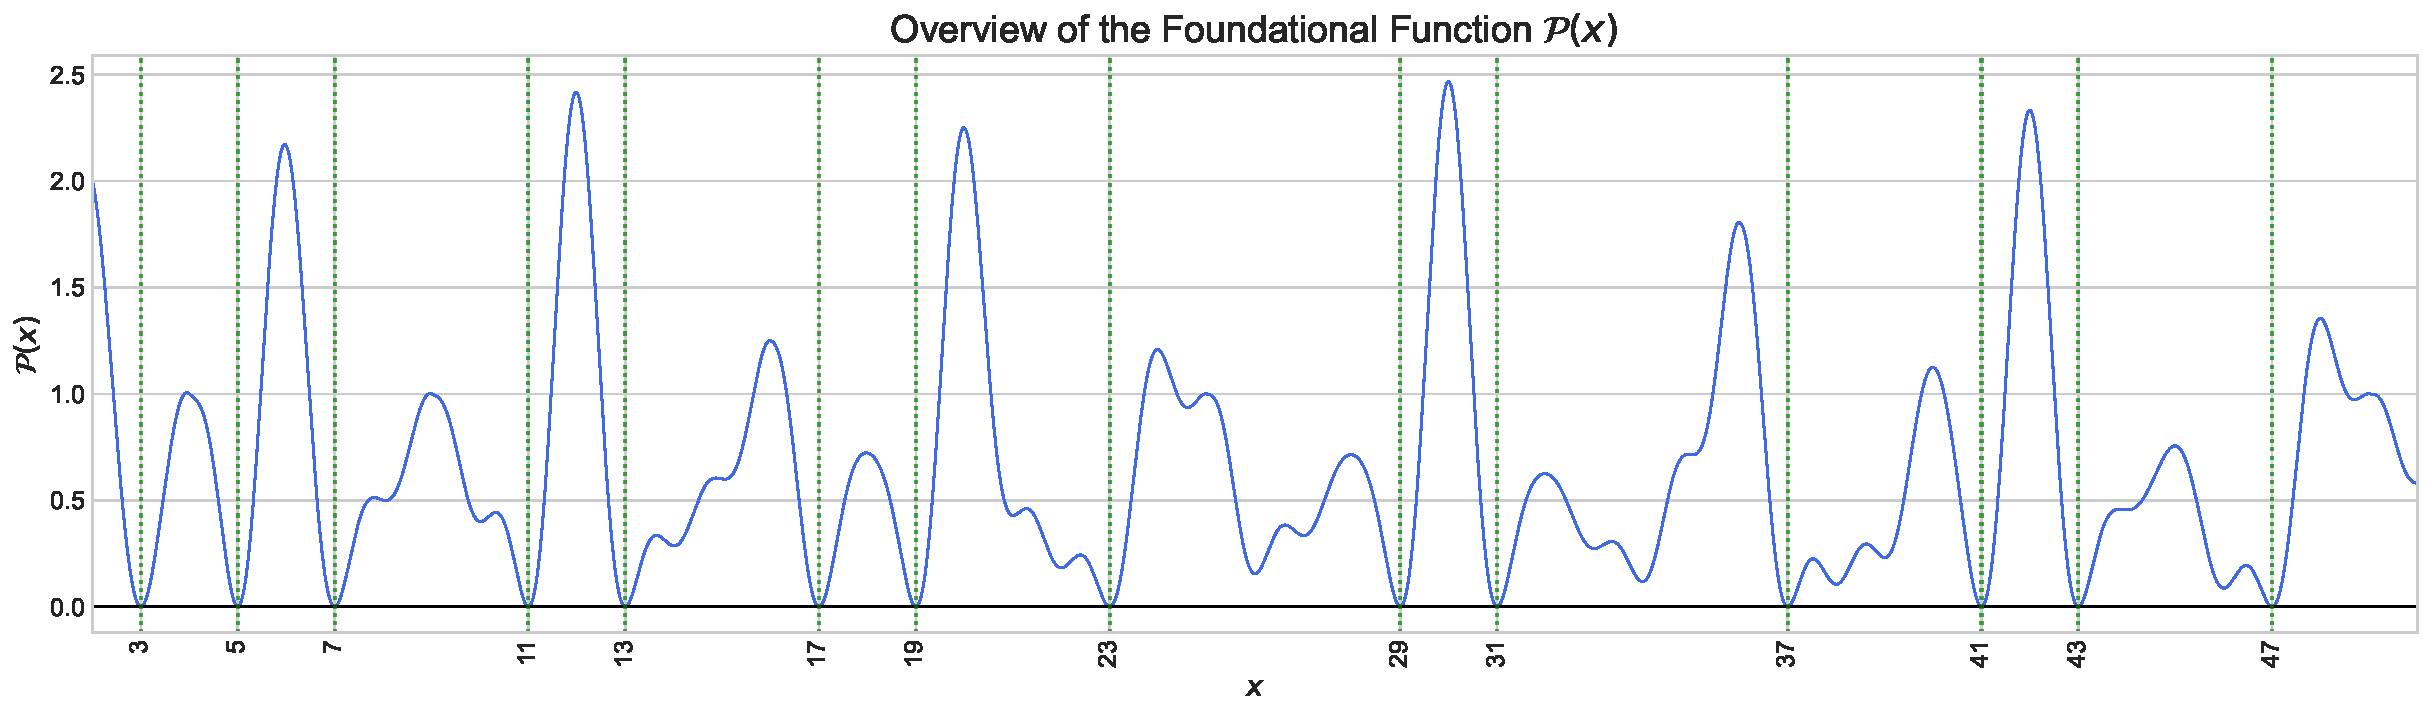
\includegraphics[width=\textwidth]{plot_overview.pdf}
\caption{Numerical profile of $\Px(x)$ for $2\le x\le 50$. Dotted vertical lines mark odd primes;
$\Px(x)$ vanishes at these positions in accordance with Theorem~\ref{thm:primezero}.}
\label{fig:overview}
\end{figure}

\begin{figure}[!htbp]
\centering
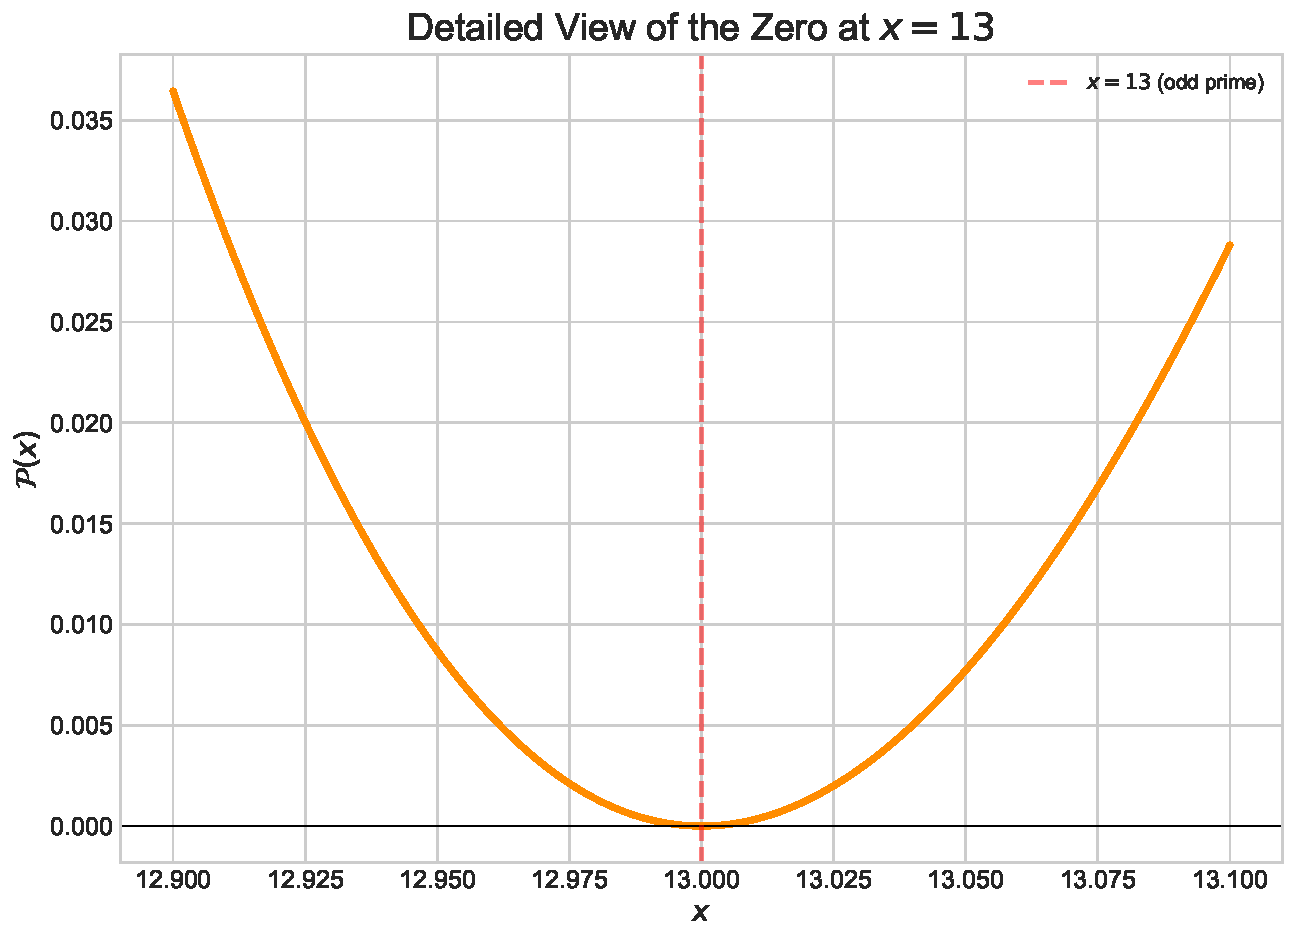
\includegraphics[width=0.8\textwidth]{plot_zoom_13.pdf}
\caption{Local behaviour of $\Px$ near $x=13$ (an odd prime).
The zero crossing illustrates the proven prime–zero property.}
\label{fig:zoom13}
\end{figure}

\begin{figure}[!htbp]
\centering
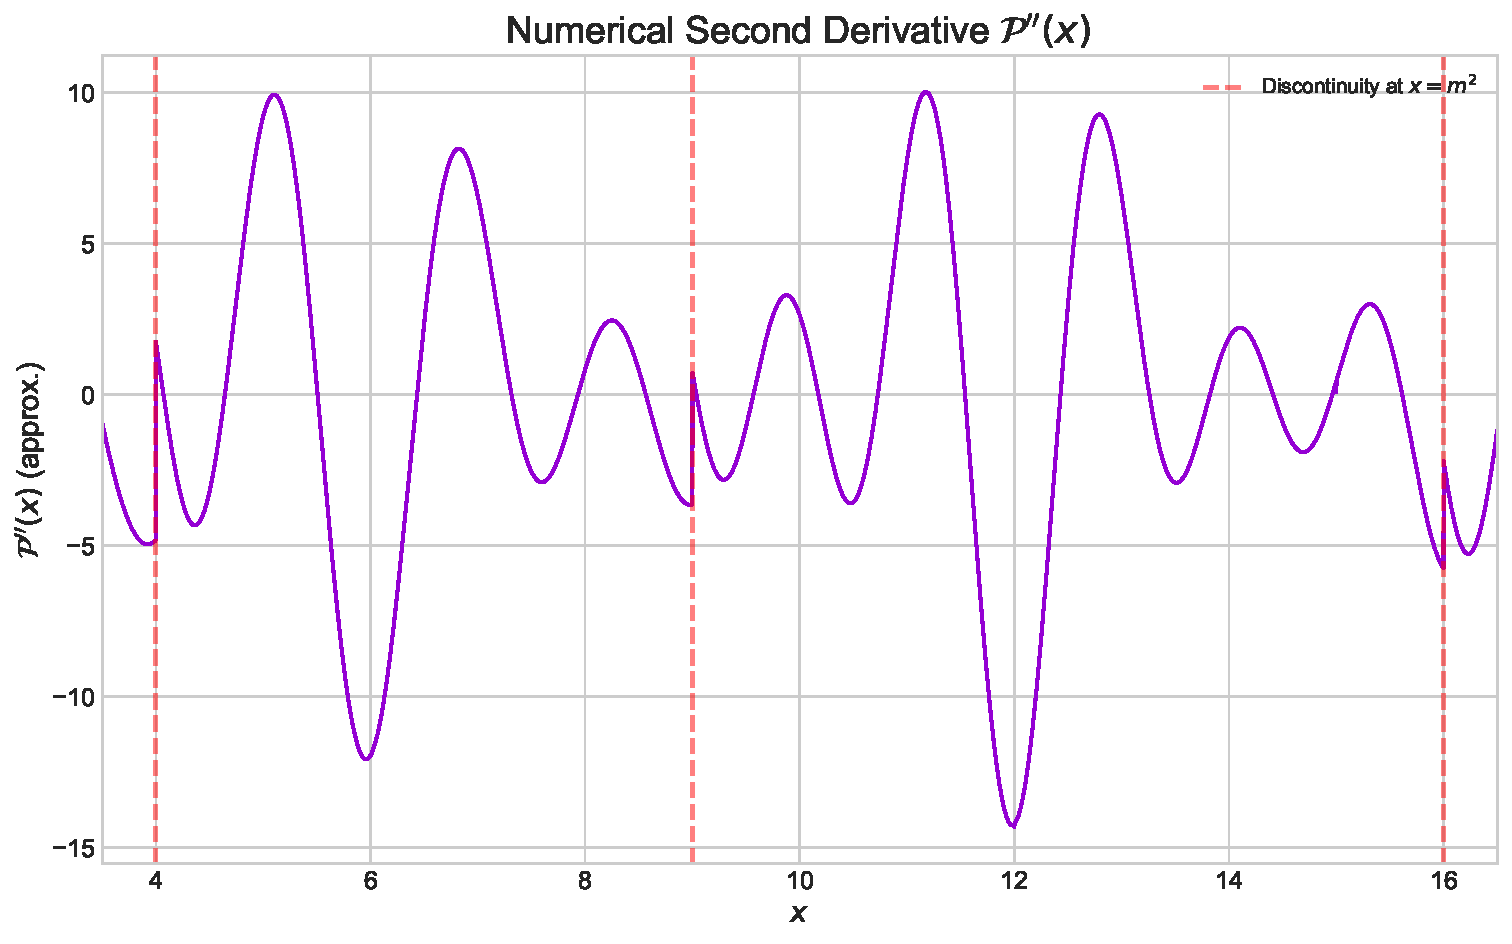
\includegraphics[width=\textwidth]{plot_second_derivative.pdf}
\caption{Finite-difference approximation of $\Px''(x)$ on $[3.5,16.5]$.
Jump discontinuities are visible at $x=4,9,16$ (integer squares), in agreement with Property~\ref{prop:second}.}
\label{fig:secondderivative}
\end{figure}

\begin{figure}[!htbp]
\centering
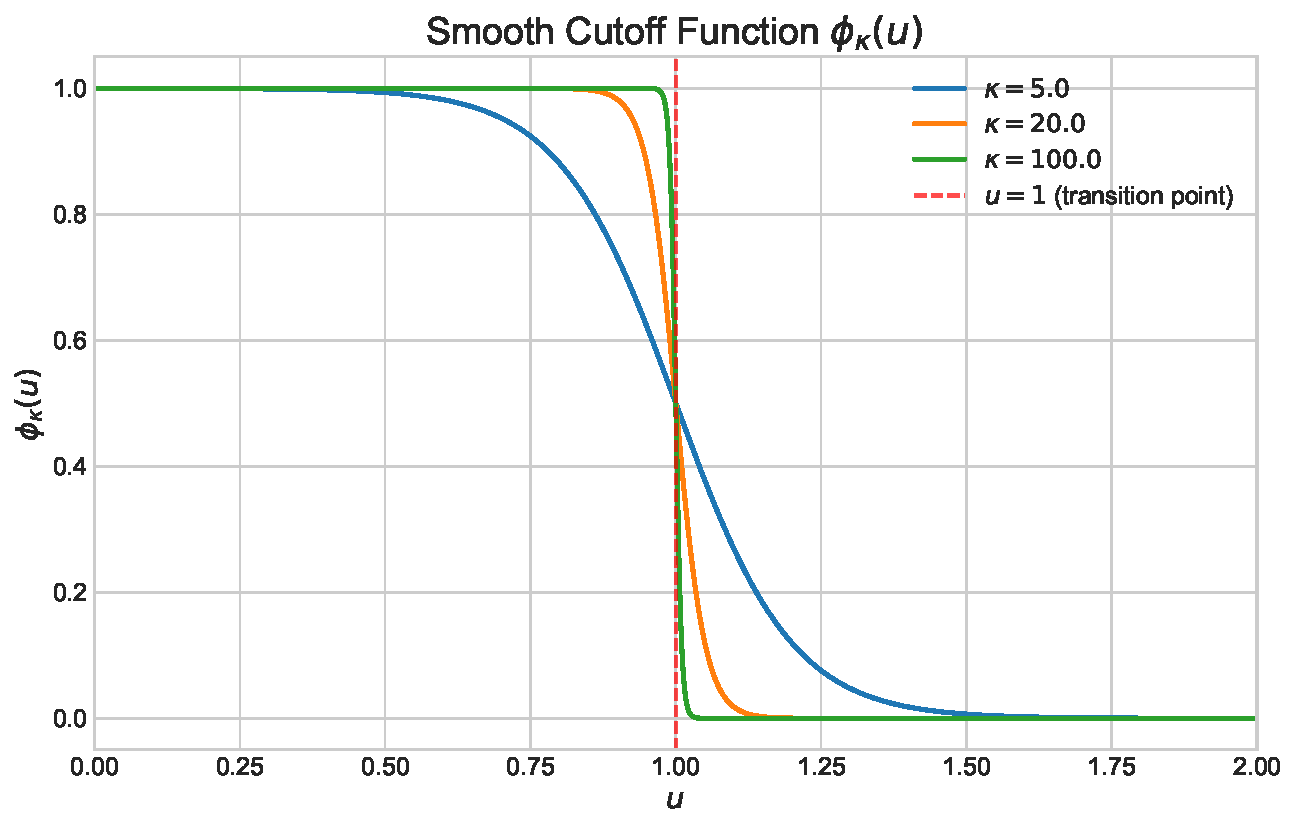
\includegraphics[width=0.8\textwidth]{plot_cutoff_function.pdf}
\caption{The smooth cutoff function $\phi_{\text{mod}}(u; k)$ for different values of the steepness parameter $k$.
The function provides a smooth transition from 1 to 0 around the point $u=1$.
Larger values of $k$ result in a sharper, more step-like transition while maintaining $C^\infty$-smoothness.}
\label{fig:cutoff}
\end{figure}

\begin{figure}[!htbp]
\centering
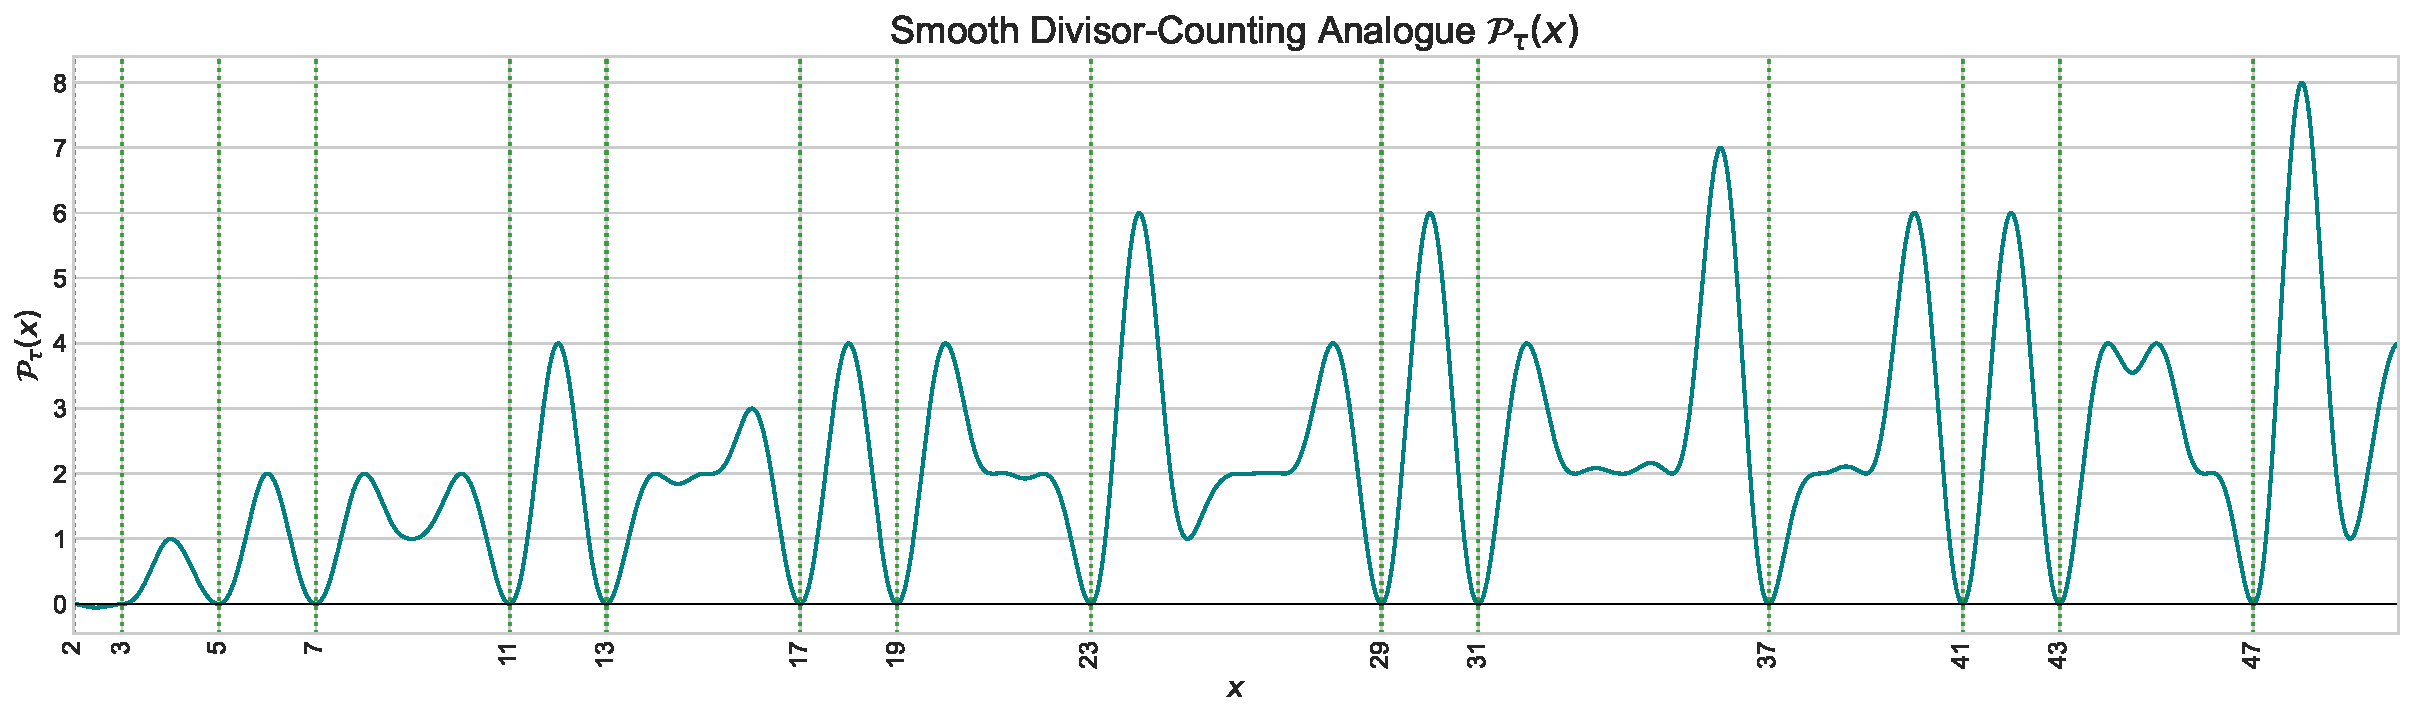
\includegraphics[width=\textwidth]{plot_P_tau.pdf}
\caption{Numerical profile of the smooth divisor-counting analogue $\Px_{\tau}(x; k)$ for $k=100$.
The function is of class $C^\infty$ and approximates zero at all prime numbers (indicated by dotted lines), including $p=2$.
For composite integers, the function's value is approximately $\tau(n)-2 > 0$.}
\label{fig:P_tau}
\end{figure}

\begin{figure}[!htbp]
\centering
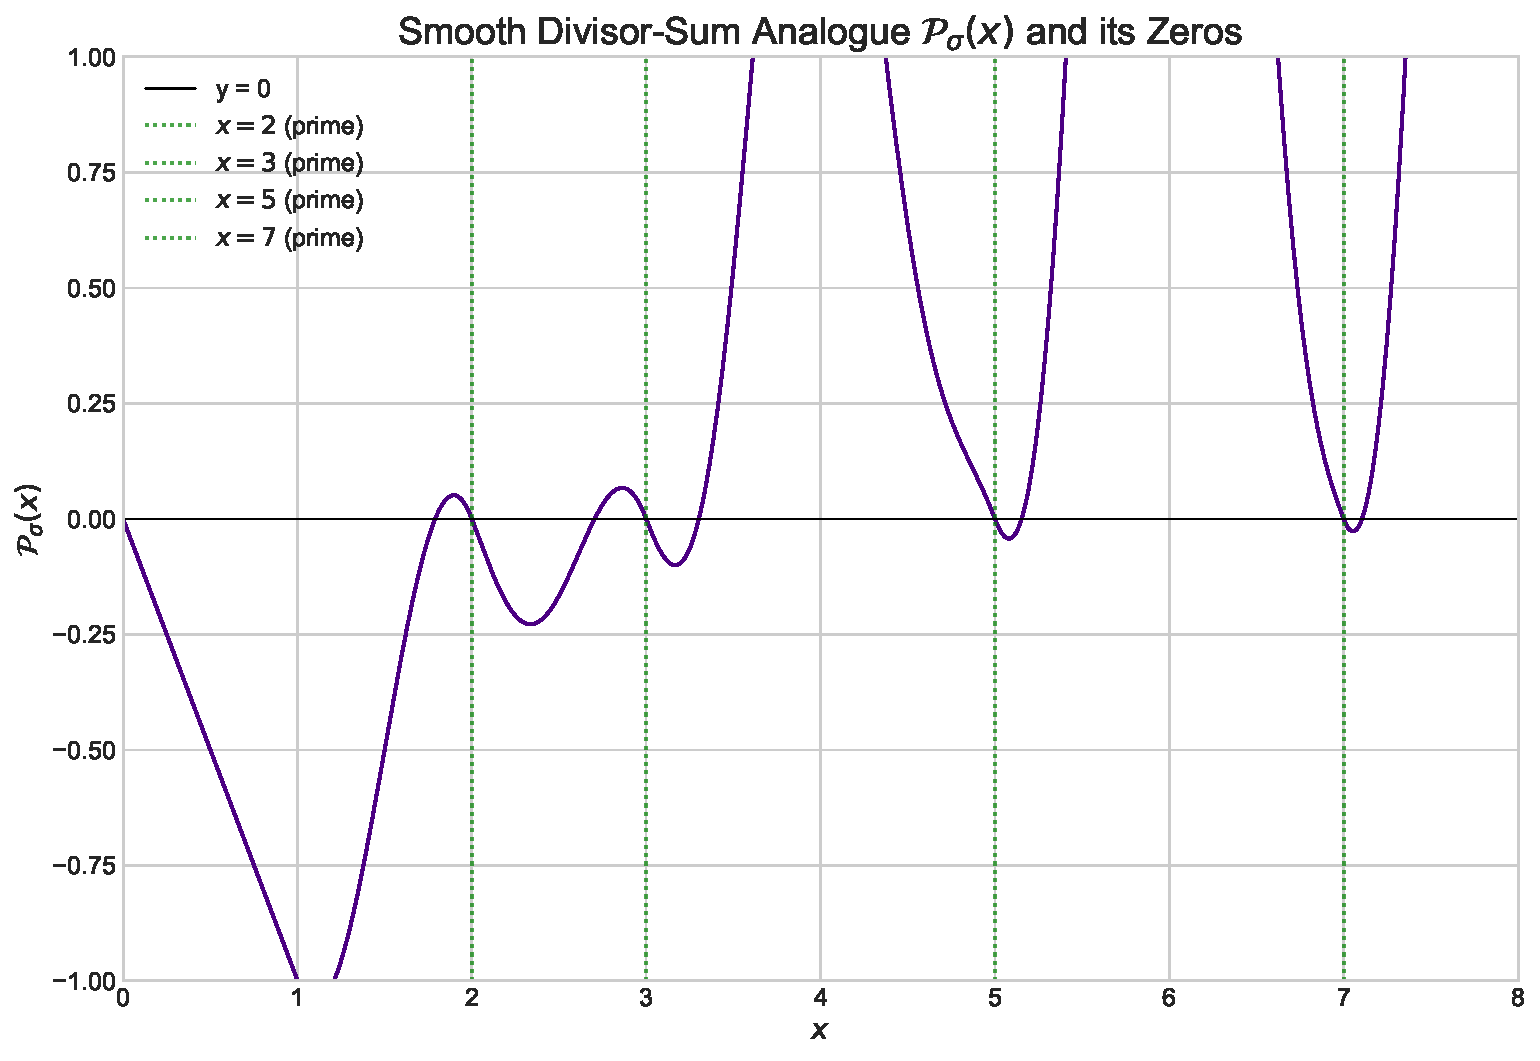
\includegraphics[width=\textwidth]{plot_P_sigma_zeros.pdf}
\caption{Behavior of the smooth divisor-sum analogue $\Px_{\sigma}(x; k)$ for $k=100$ in the interval $[0, 8]$.
The function correctly vanishes at the integer primes $2, 3, 5, 7$.
The plot illustrates the open question discussed in the text: while the function is non-zero for composite integers, its complex oscillatory behavior could theoretically allow for intersections with the x-axis at non-integer points.}
\label{fig:P_sigma}
\end{figure}

\begin{figure}[!htbp]
\centering
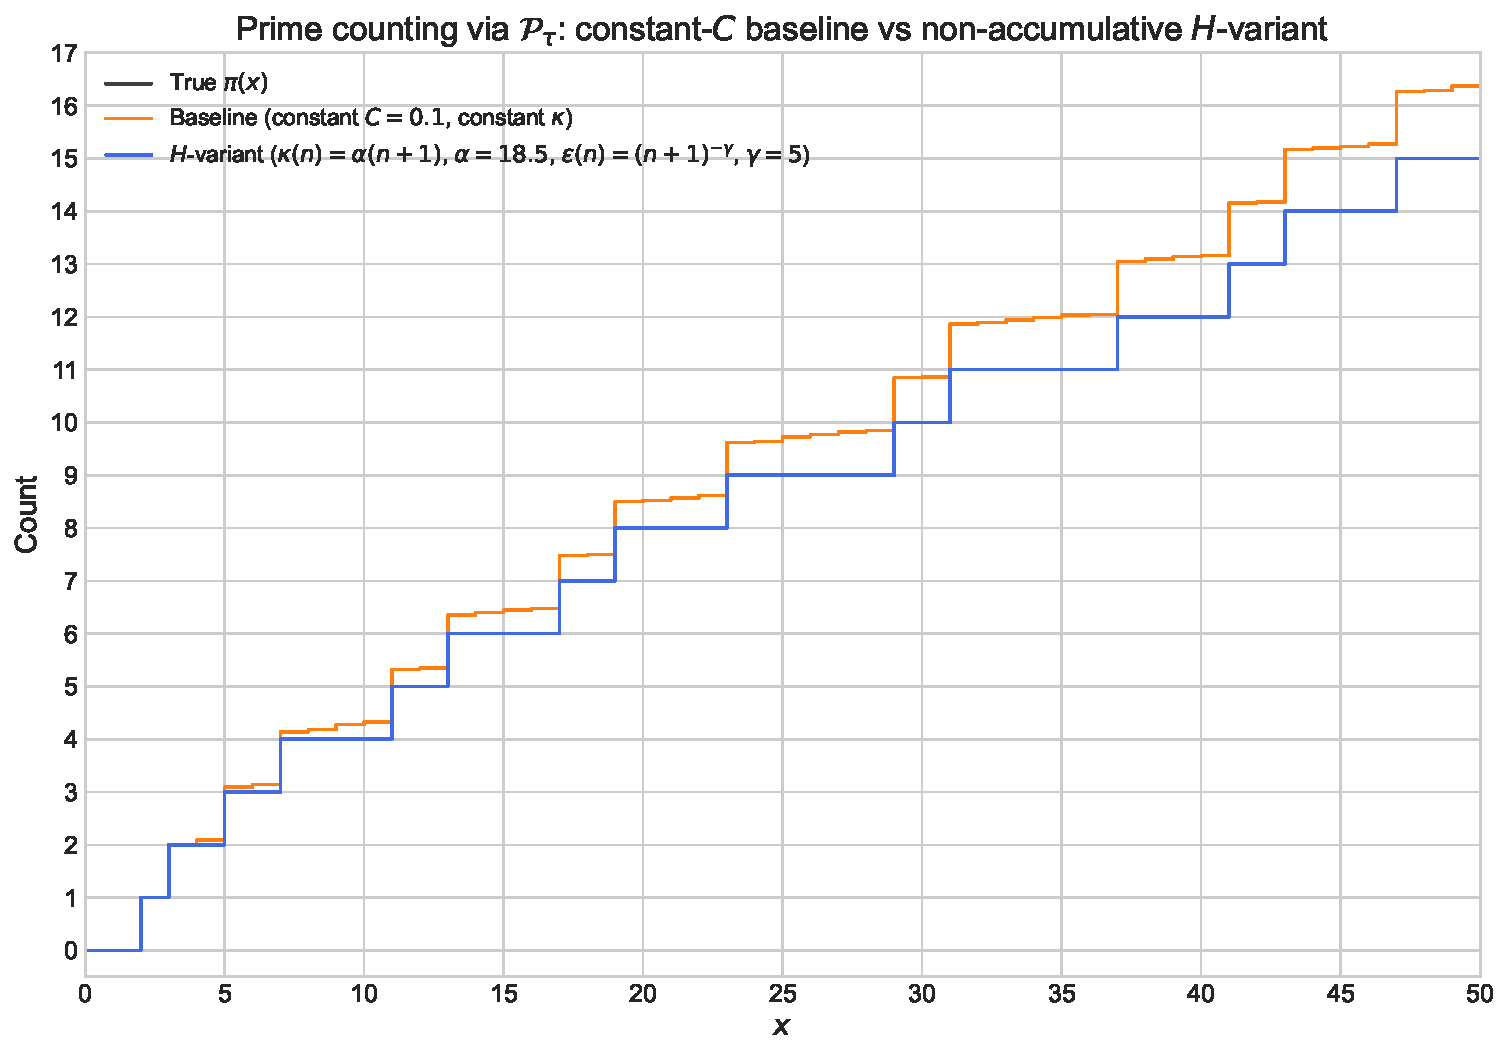
\includegraphics[width=\textwidth]{plot_prime_counting.pdf}
\caption{The step function $\pi_\Px(x; C)$ for $x\le 50$, constructed via the principles outlined.
The steps of the function align with the prime numbers, illustrating the underlying prime-zero property of the function $\Px(x)$.}
\label{fig:primecounting}
\end{figure}

% ---------------------------------------------------------------------------
\appendix
\section{Acknowledgements}
The author wishes to thank several colleagues for their insightful discussions and valuable feedback during the development of this work.
\begin{thebibliography}{13}

\bibitem{pimsCRG2024}
L.~Bellaïche, S.~J.~Lester, and A.~T.~M.~Anisha, \emph{Open Problems in Comparative Prime Number Theory}, arXiv:2407.03530 [math.NT], 2024.

\bibitem{hardy2008}
G.\,H.~Hardy and E.\,M.~Wright, \emph{An Introduction to the Theory of Numbers}, 6th ed., Oxford University Press, 2008.

\bibitem{helfgott2023}
A.~Helfgott, Analytic prime indicators revisited, \emph{Proc.\ Lond.\ Math.\ Soc.} \textbf{127} (2023), 1–29.
\bibitem{hiary2018}
G.\,B.~Hiary and N.~Hiary, An explicit prime-detecting function, \emph{J.\ Théor.\ Nombres Bordeaux} \textbf{30} (2018), 105–132.
\bibitem{iwaniec2004}
H.~Iwaniec and E.~Kowalski, \emph{Analytic Number Theory}, AMS Colloquium Publ.\ 53, 2004.

\bibitem{mazzanti2024}
S.~Mazzanti, On arithmetic terms expressing the prime-counting function and the n-th prime, \emph{arXiv:2412.14594 [math.NT]}, 2024.

\bibitem{mills1947}
W.\,H.~Mills, A prime-representing function, \emph{Bull.\ Amer.\ Math.\ Soc.} \textbf{53} (1947), 604.

\bibitem{montgomery2007}
H.\,L.~Montgomery and R.\,C.~Vaughan, \emph{Multiplicative Number Theory I: Classical Theory}, Cambridge University Press, 2007.

\bibitem{semenov2025}
S.~Semenov, A Smooth Analytical Approximation of the Prime Characteristic Function, \emph{arXiv:2504.14414 [math.GM]}, 2025.

\bibitem{seriprim2022}
E.~Seri, On analytic prime indicators, \emph{J.\ Number Theory} \textbf{162} (2022), 287–303.
\bibitem{titchmarsh1986}
E.\,C.~Titchmarsh, \emph{The Theory of the Riemann Zeta-Function}, 2nd ed., rev.
by D. R. Heath-Brown, Oxford University Press, 1986.

\bibitem{willans1964}
C.\,P.~Willans, On formulae for the $n$-th prime number, \emph{Math.\ Gazette} \textbf{48} (1964), 413–415.
\bibitem{zygmund2002}
A.~Zygmund, \emph{Trigonometric Series}, 3rd ed., Cambridge Univ.\ Press, 2002.

\end{thebibliography}

\vfill
\par\noindent
\small
Sebastian Fuchs \\[1ex]
\textit{arXiv:} \texttt{\href{https://arxiv.org/abs/2506.18933}{arXiv:2506.18933v2 [math.NT]}} \\
\textit{DOI:} \texttt{\href{https://doi.org/10.5281/zenodo.15712807}{10.5281/zenodo.15712807}} \\ 
\textit{ORCID:} \texttt{\href{https://orcid.org/0009-0009-1237-4804}{0009-0009-1237-4804}} \\

\end{document}
